\newif\ifglobal

%%%%%%%%%%%%%%%%%%%%%%%
%%% Compile to view %%%
%%%%%%%%%%%%%%%%%%%%%%%

%%%%%%%%%%%%%%%%%%%%%%%%%%%%%%%%%%%%%%%%%%%%%%%%%%%
%%% Readme:                                     %%%
%%% https://www.overleaf.com/read/bwdjvfjksvjy/ %%%
%%%%%%%%%%%%%%%%%%%%%%%%%%%%%%%%%%%%%%%%%%%%%%%%%%%

% >>> M?: marks a module setting number or important notice

% >>> M4: Set {./relative-path} to external files for this module <<<
\def \modulefiles {./13-DIGSIG}
% To add an external file, use:
% (Replace '---' with actual filename)
% '\input{\modulefiles/tables/---.tex}' for tables
% '\includegraphics{\modulefiles/figures/---}' for figures
% '\subfile{\modulefiles/---}' for register files

% >>> M1: This module is in global project? <<<
% 'YES' - uncomment; 'NO' - comment out
\globaltrue

\ifglobal
    \documentclass[main\_\_EN.tex]{subfiles}

\else
    \documentclass[openany, 10pt]{book}

    % >>> M2: In ./00-shared/preamble-trm-module, also find
    %         settings for visibility of todo notes, watermark <<<
    \usepackage{preamble-trm-module}

    % >>> M3: Temporary labels in English,
    %         you can add your own labels there <<<
    \myexternaldocument{./00-shared/temp-labels-en}

\fi %\ifglobal


\setcounter{secnumdepth}{4}

% >>> M5: If this module needs any updates in
% './00-shared/preamble-trm-module.sty'
% (include additional package, etc.), contact your module PM
% or create the file './00-shared/changelog.tex' make the
% necessary updates yourself and document them in this file <<<


\begin{document}


% Sets language into which pre-defined bits of text are translated
\selectlanguage{english}

% Do not delete this block
\ifglobal
% Add the following front matter if
% this module is outside of global project
\else
    \InputIfFileExists{readme}{}{}
    {\let\clearpage\relax \listoftodos}
    \tableofcontents
    %\listoftables
    %\listoffigures
\fi


%%%%%%%%%%%%%%%%%%%%%%%%%
%%% TRM Module Begins %%%
%%%%%%%%%%%%%%%%%%%%%%%%%

\hypertarget{digsig}{}\hypertarget{rsads}{}
\chapter{RSA Digital Signature Peripheral (RSA\_DS)}
\label{mod:digsig}

\section{Overview}

A Digital Signature is used to verify the authenticity and integrity of a message using a cryptographic algorithm. This can be used to validate a device's identity to a server, or to check the integrity of a message.

The \chipname{} includes an RSA Digital Signature Peripheral (RSA\_DS) providing hardware acceleration of messages' signatures based on RSA. It uses pre-encrypted parameters to calculate a signature. The parameters are encrypted using HMAC as a key-derivation function. In turn, the HMAC uses eFuses as an input key. The whole process happens in hardware so that neither the decryption key for the RSA parameters nor the input key for the HMAC key derivation function can be seen by the users while calculating the signature.

\section{Features}

\begin{itemize}
\item RSA Digital Signatures with key length up to 4096 bits
\item Encrypted private key data, only decryptable by the RSA\_DS peripheral
\item SHA-256 digest to protect private key data against tampering by an attacker
\end{itemize}


\section{Functional Description}
\subsection{Overview}

The RSA\_DS peripheral calculates RSA signature as \begin{math}Z = X^{Y} \bmod M\end{math} where \begin{math}Z\end{math} is the signature, \begin{math}X\end{math} is the input message, \begin{math}Y\end{math} and \begin{math}M\end{math} are the RSA private key parameters.

Private key parameters are stored in flash or other memory as ciphertext. They are decrypted using \begin{math} RSA\_DS\_KEY \end{math} which can only be read by the RSA\_DS peripheral via the HMAC peripheral. The required inputs (\begin{math} HMAC\_KEY \end{math}) to generate the key are only stored in eFuse and can only be accessed by the HMAC peripheral. The RSA\_DS peripheral hardware can decrypt the private key, and the private key in plaintext is never accessed by the software. For more detailed information about eFuse and HMAC peripherals, please refer to Chapter \ref{mod:efuse} \textit{\nameref{mod:efuse}} and \ref{mod:hmac} \textit{\nameref{mod:hmac}} peripheral.

The input message \begin{math}X\end{math} will be sent directly to the RSA\_DS peripheral by the software, each time a signature is needed. After the RSA signature operation, the signature \begin{math}Z\end{math} is read back by the software.

For better understanding, we define some symbols and functions here, which are only applicable to this chapter:

\begin{itemize}
\item
1\begin{math}^s\end{math}
\hspace{0.75cm}
A bit string consist of \begin{math}s\end{math} bits that stores ``1".

\item
    \begin{math}[x]_{s}\end{math}  \hspace{0.5cm}
       A bit string of \begin{math}s\end{math} bits, in which \begin{math}s\end{math} should be the integral multiple of 8 bits. If \begin{math}x\end{math} is a number (\begin{math}x\end{math} < 2\begin{math}^s\end{math}), it is represented in little endian byte order in the bit string. \begin{math}x\end{math} may be a variable value such as \begin{math}[Y]_{4096}\end{math} or as a hexadecimal constant such as [0x0C]\begin{math}_{8}\end{math}. If necessary, the value \begin{math}[x]_{t}\end{math} can be right-padded with \begin{math} (s-t) \end{math} number of 0 to reach \begin{math}s\end{math} bits in length, and finally get \begin{math}[x]_{s}\end{math}. For example, [0x05]\begin{math}_{8} = 00000101\end{math},
       [0x05]\begin{math}_{16} = 00000101 00000000\end{math},
       [0x0005]\begin{math}_{16} = 00000000 00000101\end{math},
       [0x13]\begin{math}_{8} = 00010011\end{math},
       [0x13]\begin{math}_{16} = 00010011 00000000\end{math},
       [0x0013]\begin{math}_{16} = 00000000 00010011\end{math}.

    \item
        \begin{math}{ || }\end{math}  \hspace{1.0cm}      A bit string concatenation operator for joining multiple bit strings into a longer bit string.
\end{itemize}



\subsection{Private Key Operands}
\label{sec:digsig-private-key-operands}

Private key operands \begin{math}Y\end{math} (private key exponent) and \begin{math}M\end{math} (key modulus) are generated by the user. They have a particular RSA key length (up to 4096 bits).
Two additional private key operands are needed: \begin{math}\overline{r}\end{math} and \begin{math}M^{\prime}\end{math}. These two operands are derived from \begin{math}Y\end{math} and \begin{math}M\end{math}.


Operands \begin{math}Y\end{math}, \begin{math}M\end{math}, \begin{math}\overline{r}\end{math} and \begin{math}M^{\prime}\end{math} are encrypted by the user along with an authentication digest and stored as a single ciphertext \begin{math}C\end{math}. \begin{math}C\end{math} is inputted to the RSA\_DS peripheral in this encrypted format, decrypted by the hardware, and then used for RSA signature calculation. Detailed description of how to generate \begin{math}C\end{math} is provided in Section \ref{sec:digsig-prerequisities}.

The RSA\_DS peripheral supports RSA signature calculation \begin{math}Z = X^{Y} \bmod M\end{math}, in which the length of operands should be \begin{math}N = 32 \times x\end{math} where \begin{math}x \in \{ 1,2,3, \dots, 128\} \end{math}. The bit lengths of arguments \begin{math}Z\end{math},
\begin{math}X\end{math},
\begin{math}Y\end{math},
\begin{math}M\end{math} and
\begin{math}\overline{r}\end{math} should be an arbitrary value in \begin{math}N\end{math}, and all of them in a calculation must be of the same length, while the bit length of \begin{math}M^{\prime}\end{math} should always be 32. For more detailed information about RSA calculation, please refer to Section \ref{sec:rsa-large-modular-Exponentiation} \textit{\nameref{sec:rsa-large-modular-Exponentiation}} in Chapter \ref{mod:rsa} \textit{\nameref{mod:rsa}}.


\subsection{Software Prerequisites}
\label{sec:digsig-prerequisities}

The left side of Figure \ref{fig:digsig-flow} lists preparations required by the software before the hardware starts RSA signature calculation, while the right side lists the hardware workflow during the entire calculation procedure.

\begin{figure}[H]
    \centering
    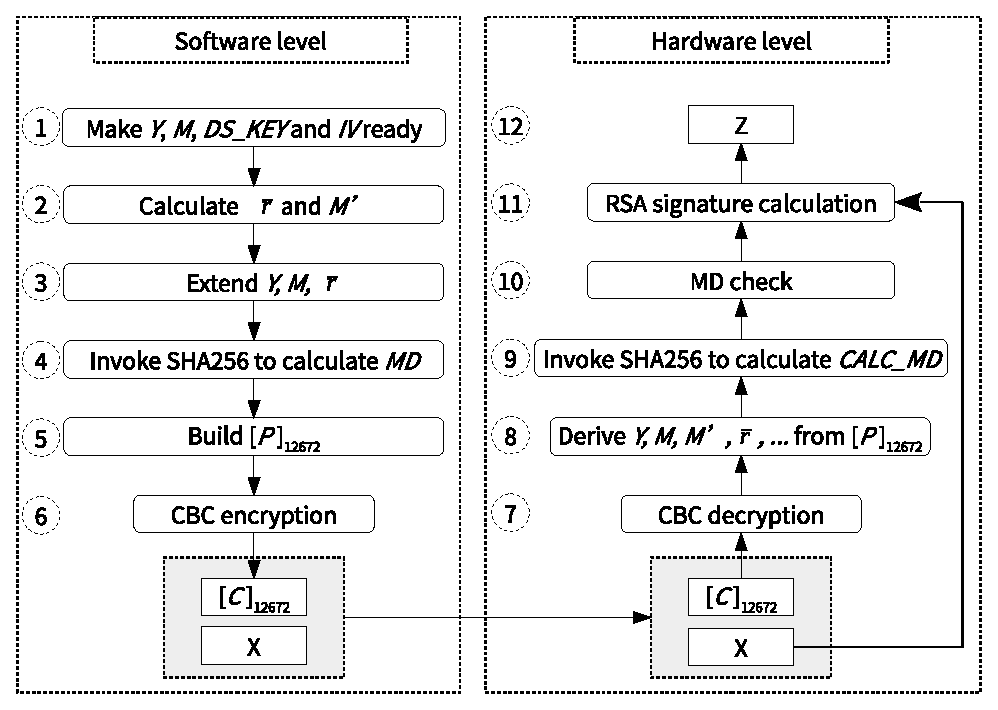
\includegraphics[width=0.7\textwidth]{./13-DIGSIG/figures/13-DIGSIG-flow__EN}
    \caption{Software Preparations and Hardware Working Process}
    \label{fig:digsig-flow}
\end{figure}


\begin{tiplisting}
\vspace{-2.5em}
\begin{enumerate}
\item The software preparation (left side in the Figure \ref{fig:digsig-flow}) is a one-time operation before any signature is calculated, while the hardware calculation (right side in the Figure 1-1) repeats for every signature calculation.
\end{enumerate}
\end{tiplisting}


Users need to follow the steps shown in the left part of Figure \ref{fig:digsig-flow} to calculate \begin{math}C\end{math}. Detailed instructions are as follows:

\begin{itemize}

    \item {\bfseries Step 1}: Prepare operands \begin{math}Y\end{math} and \begin{math}M\end{math} whose lengths should meet the requirements in Section \ref{sec:digsig-private-key-operands}. Define \begin{math}[L]_{32} = \frac{N}{32}-1 \end{math} (i.e., for RSA 4096, \begin{math}[L]_{32}\end{math} == [0x80-1]\begin{math}_{32}\end{math}). Prepare \begin{math}[HMAC\_KEY]_{256}\end{math} and calculate \begin{math}[RSA\_DS\_KEY]_{256}\end{math} based on \begin{math}RSA\_DS\_KEY\end{math} = HMAC-SHA256 (\begin{math}[HMAC\_KEY]_{256}\end{math}, \begin{math}1^{256}\end{math}). Generate a random \begin{math}[IV]_{128}\end{math} which should meet the requirements of the AES-CBC block encryption algorithm. For more information on AES, please refer to Chapter \ref{mod:aes} \textit{\nameref{mod:aes}}.

    \item {\bfseries Step 2}: Calculate \begin{math}\overline{r}\end{math} and \begin{math}M^{\prime} \end{math} based on \begin{math}M\end{math}.


    \item {\bfseries Step 3}: Extend \begin{math}Y\end{math}, \begin{math}M\end{math} and \begin{math}\overline{r}\end{math}, in order to get \begin{math}[Y]_{4096}\end{math}, \begin{math}[M]_{4096}\end{math} and \begin{math}[\overline{r}]_{4096}\end{math}, respectively. This step is only required for \begin{math}Y\end{math}, \begin{math}M\end{math} and \begin{math}\overline{r}\end{math} whose length are less than 4096 bits, since their largest length are 4096 bits.


    \item {\bfseries Step 4}: Calculate MD authentication code using the SHA-256: \\
    \begin{math}[MD]_{256}\end{math} = SHA256 (
            \begin{math}
                [Y]_{4096} ||
                [M]_{4096} ||
                [\overline{r}]_{4096} ||
                [M^{\prime}]_{32} ||
                [L]_{32} ||
                [IV]_{128}
            \end{math})

    \item {\bfseries Step 5}: Build \begin{math}[P]_{12672}\end{math} = (
            \begin{math}
                [Y]_{4096} ||
                [M]_{4096} ||
                [\overline{r}]_{4096} ||
                [MD]_{256} ||
                [M^{\prime}]_{32} ||
                [L]_{32} ||
                [\beta]_{64})
            \end{math}, where \begin{math}[\beta]_{64} \end{math} is a PKCS\#7 padding value, i.e., a 64-bit string $[$0x0808080808080808$]_{64}$ composed of 8 bytes (value = 0x80). The purpose of \begin{math}[\beta]_{64} \end{math} is to make the bit length of \begin{math}P\end{math} a multiple of 128.

    \item {\bfseries Step 6}: Calculate \begin{math}C\end{math} = \begin{math}[C]_{12672}\end{math} =
            AES-CBC-ENC (\begin{math}[P]_{12672}\end{math}, \begin{math}[RSA\_DS\_KEY]_{256}\end{math}, \begin{math}[IV]_{128}\end{math}), where \begin{math}C\end{math} is the ciphertext with length of 12672 bits.
\end{itemize}


\subsection{RSA\_DS Operation at the Hardware Level}
\label{sec:digsig-operation-at-the-hardware-level}

The hardware operation is triggered each time a digital signature needs to be calculated. The inputs are the pre-generated private key ciphertext \begin{math}C\end{math}, a unique message \begin{math}X\end{math}, and \begin{math}IV\end{math}.

The RSA\_DS operation at the hardware level can be divided into the following three stages:

\begin{enumerate}

    \item {\bfseries Decryption: Step 7 and 8 in Figure \ref{fig:digsig-flow}}


        The decryption process is the inverse of Step 6 in figure \ref{fig:digsig-flow}. The RSA\_DS peripheral will call AES accelerator to decrypt \begin{math}C\end{math} in CBC block mode and get the resulted plaintext. The decryption process can be represented by \begin{math}P\end{math} = AES-CBC-DEC (\begin{math}C\end{math}, \begin{math}RSA\_DS\_KEY\end{math}, \begin{math}IV\end{math}), where \begin{math}IV\end{math} (i.e., \begin{math}[IV]_{128}\end{math}) is defined by users. \begin{math}[RSA\_DS\_KEY]_{256}\end{math} is provided by HMAC module, derived from \begin{math}HMAC\_KEY\end{math} stored in eFuse. \begin{math}[RSA\_DS\_KEY]_{256}\end{math}, as well as \begin{math}[HMAC\_KEY]_{256}\end{math} are not readable by users. For more information, please refer to Chapter \ref{mod:hmac} \textit{\nameref{mod:hmac}}.

        With P, the RSA\_DS peripheral can derive \begin{math}[Y]_{4096}\end{math}, \begin{math}[M]_{4096}\end{math}, \begin{math}[\overline{r}]_{4096}\end{math}, \begin{math}[M^{\prime}]_{32}\end{math}, \begin{math}[L]_{32}\end{math}, MD authentication code, and the padding value \begin{math}[\beta]_{64} \end{math}. This process is the inverse of Step 5.

    \item {\bfseries Check: Step 9 and 10 in Figure \ref{fig:digsig-flow}}

        The RSA\_DS peripheral will perform two checks: MD check and padding check. Padding check is not shown in Figure \ref{fig:digsig-flow}, as it happens at the same time with MD check.


        \begin{itemize}

            \item MD check: The RSA\_DS peripheral calls SHA-256 to calculate the MD authentication code \begin{math}[CALC\_MD]_{256}\end{math} from \begin{math}
                [Y]_{4096} ||
                [M]_{4096} ||
                [\overline{r}]_{4096} ||
                [M^{\prime}]_{32} ||
                [L]_{32} ||
                [IV]_{128}
            \end{math}). Then, \begin{math}[CALC\_MD]_{256}\end{math} is compared against the pre-calculated MD authentication code \begin{math}[MD]_{256}\end{math} from step 4. Only when the two match, MD check passes.

            \item Padding check: The RSA\_DS peripheral checks if \begin{math}[\beta]_{64} \end{math} complies with the aforementioned PKCS\#7 format. Only when \begin{math}[\beta]_{64} \end{math} complies with the format, padding check passes.

        \end{itemize}

        The RSA\_DS peripheral will only perform subsequent operations if MD check passes. If padding check fails, an error bit is set in the query register, but it does not affect the subsequent operations, i.e., it is up to the user to proceed or not.

    \item {\bfseries Calculation: Step 11 and 12 in Figure \ref{fig:digsig-flow}}

        The RSA\_DS peripheral treats \begin{math}X\end{math} (input by users) and \begin{math}Y\end{math}, \begin{math}M\end{math}, \begin{math}\overline{r}\end{math} (compiled) as big numbers. With \begin{math}M^{\prime}\end{math}, all operands to perform \begin{math} X^{Y} \bmod M\end{math} are in place. The operand length is defined by \begin{math}L\end{math}. The RSA\_DS peripheral will get the signed result \begin{math}Z\end{math} by calling RSA to perform \begin{math}Z = X^{Y} \bmod M\end{math}.

\end{enumerate}


\subsection{RSA\_DS Operation at the Software Level}

The following software steps should be followed each time an RSA\_DS signature needs to be calculated. The inputs are the pre-generated private key ciphertext \begin{math}C\end{math}, a unique message \begin{math}X\end{math}, and \begin{math}IV\end{math}. These software steps trigger the hardware steps described in Section \ref{sec:digsig-operation-at-the-hardware-level}.

We assume that the software has called the HMAC peripheral and HMAC on the hardware has calculated \begin{math}RSA\_DS\_KEY\end{math} based on \begin{math}HMAC\_KEY\end{math}.

\begin{enumerate}

    \item {\bfseries Prerequisites}: Prepare operands \begin{math}C\end{math}, \begin{math}X\end{math}, \begin{math}IV\end{math} according to Section \ref{sec:digsig-prerequisities}.

    \item {\bfseries Activate the RSA\_DS peripheral}: Write 1 to \hyperref[regdesc:DSSETSTARTREG]{DS\_SET\_START\_REG}.

    \item {\bfseries Check if \begin{math}RSA\_DS\_KEY\end{math} is ready}: Poll \hyperref[regdesc:DSQUERYBUSYREG]{DS\_QUERY\_BUSY\_REG} until the software reads 0.

    If the software does not read 0 in \hyperref[regdesc:DSQUERYBUSYREG]{DS\_QUERY\_BUSY\_REG} after approximately 1 ms, it indicates a problem with HMAC initialization. In such a case, the software can read register \hyperref[regdesc:DSQUERYKEYWRONGREG]{DS\_QUERY\_KEY\_WRONG\_REG} to get more information:

    \begin{itemize}

        \item If the software reads 0 in \hyperref[regdesc:DSQUERYKEYWRONGREG]{DS\_QUERY\_KEY\_WRONG\_REG}, it indicates that the HMAC peripheral has not been activated.

        \item If the software reads any value from 1 to 15 in \hyperref[regdesc:DSQUERYKEYWRONGREG]{DS\_QUERY\_KEY\_WRONG\_REG}, it indicates that HMAC was activated, but the RSA\_DS peripheral did not successfully receive \begin{math}RSA\_DS\_KEY\end{math} from the HMAC peripheral. This may indicate that the HMAC operation has been interrupted due to a software concurrency problem.

    \end{itemize}

    \item {\bfseries Configure register}: Write \begin{math}IV\end{math} block to register DS\_IV\_\textcolor{red}{\it{m}}\_REG (\textcolor{red}{\it{m}}: 0-3). For more information on the \begin{math}IV\end{math} block, please refer to Chapter \ref{mod:aes} \textit{\nameref{mod:aes}}.

    \item {\bfseries Write \begin{math}X\end{math} to memory block \hyperref[DSXMEM]{DS\_X\_MEM}}: Write \begin{math}X_{i}\end{math}
        (\begin{math}i \in \{ 0, 1, \dots, n-1 \} \end{math}), where \begin{math} n = \frac{N}{32} \end{math}, to memory block \hyperref[DSXMEM]{DS\_X\_MEM} whose capacity is 128 words. Each word can store one base-\begin{math}b\end{math} digit. The memory block uses the little endian format for storage, i.e., the least significant digit of the operand is in the lowest address. Words in \hyperref[DSXMEM]{DS\_X\_MEM} block after the configured length of \begin{math}X\end{math} (\begin{math}N\end{math} bits, as described in Section \ref{sec:digsig-private-key-operands}) are ignored.

    \item {\bfseries Write \begin{math}C\end{math} to memory block \hyperref[DSCMEM]{DS\_C\_MEM}}: Write \begin{math}C_{i}\end{math}
        (\begin{math}i \in \{ 0, 1, \dots, 395 \} \end{math})
        to memory block \hyperref[DSCMEM]{DS\_C\_MEM} whose capacity is 396 words. Each word can store one base-\begin{math}b\end{math} digit.


    \item {\bfseries Start RSA\_DS operation}: Write 1 to register \hyperref[regdesc:DSSETMEREG]{DS\_SET\_ME\_REG}.

    \item {\bfseries Wait for the operation to be completed}: Poll register \hyperref[regdesc:DSQUERYBUSYREG]{DS\_QUERY\_BUSY\_REG} until the software reads 0.

    \item {\bfseries Query check result}: Read register \hyperref[regdesc:DSQUERYCHECKREG]{DS\_QUERY\_CHECK\_REG} and determine the subsequent operations based on the return value.

    \begin{itemize}

        \item If the value is 0, it indicates that both padding check and MD check pass. Users can continue to get the signed result \begin{math}Z\end{math}.

        \item If the value is 1, it indicates that the padding check passes but MD check fails. The signed result \begin{math}Z\end{math} is invalid. The operation will resume directly from Step \ref{other:digsig-step-exit}.

        \item If the value is 2, it indicates that the padding check fails but MD check passes. Users can continue to get the signed result \begin{math}Z\end{math}. But please note that the data encapsulation format does not comply with the aforementioned PKCS\#7 format, which may not be what you want.

        \item If the value is 3, it indicates that both padding check and MD check fail. In this case, some fatal errors may occurred and the signed result \begin{math}Z\end{math} is invalid. The operation will resume directly from Step \ref{other:digsig-step-exit}.

    \end{itemize}

    \item {\bfseries Read the signed result}: Read the signed result \begin{math}Z_{i}\end{math} (\begin{math}i \in \{0,1,\dots,n-1\}\end{math}), where \begin{math} n = \frac{N}{32} \end{math}, from memory block \hyperref[DSZMEM]{DS\_Z\_MEM}. The memory block stores \begin{math}Z\end{math} in little-endian byte order.

    \item {\bfseries Exit the operation\label{other:digsig-step-exit}}: Write 1 to \hyperref[regdesc:DSSETFINISHREG]{DS\_SET\_FINISH\_REG}, then poll \hyperref[regdesc:DSQUERYBUSYREG]{DS\_QUERY\_BUSY\_REG} until the software reads 0.

\end{enumerate}

After the operation, all the input/output registers and memory blocks are cleared.

\clearpage
\section{ Memory Summary}
\label{sec:digsig-mem-summ}

The addresses in this section are relative to the RSA Digital Signature Peripheral (RSA\_DS) base address provided in Table \ref{tab:sysmem-base-address} in Chapter \ref{mod:sysmem} \textit{\nameref{mod:sysmem}}.

\subfile{\modulefiles/13-DIGSIG-mem-summ__EN}

%%%%%%%%%%%%%%%%%%%%%%%%
%%% Register Summary %%%
%%%%%%%%%%%%%%%%%%%%%%%%

% >>> Update the sample text below and insert
%     the info on register summary into the subfile <<<

\clearpage
\section{Register Summary}
\label{sec:digsig-reg-summ}
\hypertarget{digsig-reg-summ}{}

The addresses in this section are relative to the RSA Digital Signature Peripheral (RSA\_DS) base address provided in Table \ref{tab:sysmem-base-address} in Chapter \ref{mod:sysmem} \textit{\nameref{mod:sysmem}}.

The abbreviations given in Column \textbf{Access} are explained in Section \hyperref[glossary-access-types]{\textit{Access Types for Registers}}.

\subfile{\modulefiles/13-DIGSIG-reg-summ__EN}


%%%%%%%%%%%%%%%%%
%%% Registers %%%
%%%%%%%%%%%%%%%%%

% >>> Update the sample text below and insert
%      the info on registers into the subfile <<<

\clearpage
\section{Registers}

The addresses in this section are relative to the RSA Digital Signature Peripheral (RSA\_DS) base address provided in Table \ref{tab:sysmem-base-address} in Chapter \ref{mod:sysmem} \textit{\nameref{mod:sysmem}}.

\subfile{\modulefiles/13-DIGSIG-reg__EN}

\end{document}
